\section{题目分析与基本假设}
题目内容如下:
\textit{
    宏观系统从任意初态通过驰豫过程演化到内秉平衡态是有条件的,所需的条件是系统必须被束缚在有限的容器内。从物理上看,这相当于要求将宏观系统放置在具有有限体积的紧闭无限深势阱内部。若将系统放置在一个并非完全禁闭的势阱内,例如置于引力场中(势函数在无限远处趋于平坦,非禁闭),试研究相应的驰豫过程所对应的非平衡演化。对这样的系统是否可以建立相应的涨落定理以及涨落耗散定理?
    }

首先,在  D  维空间中,我们考虑一个在无穷远处趋于0且各向同性的单势阱,故在球坐标下势能  $V(r)$  随径向坐标$r$  变化图像大致如下图所示:
\begin{figure}[htbp]
  \centering
  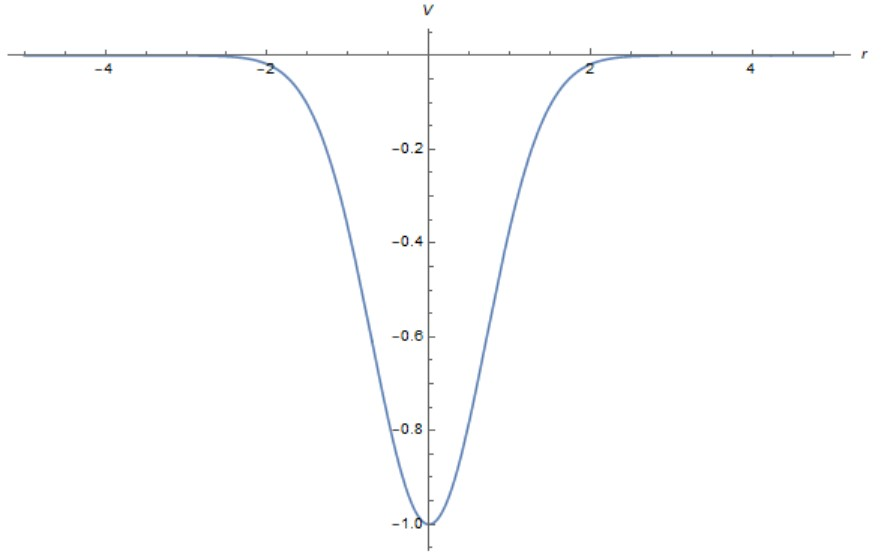
\includegraphics[width=0.8\linewidth]{figs/potential.jpg}
  \caption{势能  $V(r)$  的示意图}
\end{figure}

当  $V(r)$  为有限深方势阱时,我们可以自然地定义势阱的边界。当  $V(r)$  是光滑函数,我们可以人为地取某个函数固定的势能值  $V_{0}$,并认为当粒子势能小于  $V_{0}$  时,粒子处于势阱内。这样,势阱内的粒子构成一个开放系。

为了方便解决问题,我们引入如下两个假设:

\textbf{1.假设存在一个足够大的孤立系,使得系统总粒子数和能量守恒。}

我们在处理开放系时,都是将开放系置于一个外界大热库中,并认为开放系与大热库一起组成一个孤立系。当粒子可以达到无穷远处时,这样的处理并不显然。但考虑到我们可以观测的时空范围是有限的,上述假设总是合理的。而且,因为我们测量能量时的分辨率是有限的,所以我们总可以找到一个足够大的空间,使得内部的能量也是守恒的。

\textbf{2.假设孤立总系存在一个内禀平衡态,且系统会自发向内禀平衡态演化。}

对于一个粒子可以达到无穷远的系统,平衡态未必存在,这依赖于势能衰减的速度,在势能衰减不够快的情况下,粒子可能都驰豫到无穷远处。在我们的讨论中,假设系统存在平衡态。并且,根据后文数值模拟的结果,在长时间近似下,势场中的粒子分布基本不发生改变,故上述假设是合理的。

此外,为了简单起见,我们只考虑经典系统,满足玻尔兹曼近似$N\rightarrow\infty$。